\documentclass[a4paper]{article}
%% Sets page size and margins
\usepackage[a4paper,top=3cm,bottom=3cm,left=3cm,right=3cm,marginparwidth=1.75cm]{geometry}
%% Useful packages
\usepackage{amsmath,amsthm,amssymb,amsfonts}
\usepackage{graphicx}
\usepackage[colorinlistoftodos]{todonotes}
\usepackage{bbm}
\usepackage{setspace}
\usepackage{footmisc}
\usepackage{pdflscape}
\usepackage{natbib}
\usepackage{booktabs}
\usepackage{caption}
\usepackage{subcaption}
\usepackage{changepage}
\usepackage{rotating}
\usepackage{bm}
\usepackage{tikz}
\usetikzlibrary{fit,tikzmark}  
\usetikzlibrary{shapes.geometric, arrows}
\usepackage{color, colortbl}

\usepackage{graphicx}
\usepackage[colorlinks=true, allcolors=blue]{hyperref}
\usepackage{url}

\renewcommand\footnotelayout{\fontsize{10}{12}\selectfont}


\tikzstyle{start} = [rectangle, rounded corners, 
minimum width=3cm, 
minimum height=1cm,
text centered, 
draw=black, 
fill=orange!30]

\tikzstyle{process} = [rectangle, 
minimum width=3cm, 
minimum height=1cm, 
text centered, 
text width=3cm, 
draw=black, 
fill=blue!30]

\tikzstyle{stop} = [rectangle, rounded corners, 
minimum width=3cm, 
minimum height=1cm,
text centered, 
draw=black, 
fill=green!30]

\tikzstyle{arrow} = [thick,->,>=stealth]



\interfootnotelinepenalty=10000

\newcommand{\R}{\mathbb{R}}
\newcommand{\N}{\mathbb{N}}
\newcommand{\Z}{\mathbb{Z}}
\providecommand{\C}{\mathbb{C}}

\theoremstyle{definition}
\newtheorem{defin}{Definição}

\theoremstyle{plain}
\newtheorem{theorem}[defin]{Teorema}
\newtheorem{corollary}[defin]{Corolário}

\linespread{2}
\title{Rawls For Electricity Planning Models}

\author{Lauren Beatty\thanks{Environmental Defense Fund  \hspace{.5cm} E-mail: lbeatty1@edf.org \hspace{.5cm}Website: \href{https://lbeatty1.github.io}{https://lbeatty1.github.io}}\\
Matthias Fripp\thanks{Energy Innovations}}

\date{\today}

\begin{document}
\maketitle
\begin{center}
    PRELIMINARY DRAFT - PLEASE DO NOT CITE OR DISTRIBUTE
\end{center}

\begin{abstract}
Renewed interest in the distributional impacts of policies require going beyond typical methods of analysis such as benefit-cost analysis.  In this paper we show how to use least-cost electricity planning models to design equitable systems by modifying their objective functions.  Rather than using the models to minimize costs, we provide the model with a min-max objective function on the distributional health effects of electricity generation and subject the solution to a total cost constraint.  This method provides a menu of plans that equitably reduce pollution exposure. Our model results show that a modest $\$$50 billion investment through 2050 could approximately cut mean air pollution exposures in half and generate the largest reductions for groups with the highest baseline exposures.
\end{abstract}


\newpage
\section{Introduction}
Mitigating climate change requires deep cuts in greenhouse gas emissions from the electricity sector. Least-cost electricity planning models have become essential tools for policymakers and utility planners seeking cost-effective generation portfolios that meet reliability requirements and emissions goals.

However, these models often ignore external costs associated with electricity generation—especially the health damages from local air pollution. Air pollution from fossil fuel combustion has been linked to a wide range of adverse health outcomes, including chronic obstructive pulmonary disease (COPD), cerebrovascular disease, ischemic heart disease, and lung cancer. In the U.S., \citet{Lelieveld2015TheScale} estimate that power generation contributes to 31$\%$ of premature mortality caused by outdoor air pollution.

These harms are not evenly distributed. Numerous studies, including \citet{Thind2019FineGeography}, show that pollution exposure varies substantially across racial and socioeconomic groups. In the U.S., Black and white populations are exposed to higher pollution levels than other groups, and low-income populations face disproportionately high exposure, even after controlling for race. These disparities raise important equity concerns as the energy system transitions away from fossil fuels.

Some prior studies have quantified the health co-benefits of decarbonization by monetizing pollution damages and incorporating them into the objective function of least-cost planning models \citep{Sergi2020OptimizingBenefits}). Others have explored how the electricity transition will affect the spatial distribution of air pollution and its consequences (\citet{Shawhan2024PoliciesAmericans}; \citet{Goforth2022AirStrategies}).

This paper takes a different approach. Instead of modifying the objective function to internalize monetized pollution damages, or analyzing expected health outcomes ex-post, we propose a new framework that endogenizes pollution exposure in the planning model and places distributional equity at the center of the optimization. Drawing inspiration from Rawlsian principles of justice, we formulate a min-max optimization in which the social planner minimizes the maximum pollution exposure across population groups, subject to an overall cost constraint. To do this, we use a reduced-form emissions to concentration model, InMAP, to calculate how much each unit of electricity generation in each model region affects population-weighted pollution exposure. Then, we use a least-cost electricity planning model, Switch, to solve for electricity system designs that achieve low pollution levels.

By solving this model at varying cost levels, we produce a set of frontier solutions that answer questions such as: How much can we equitably reduce pollution exposure for $\$$100 billion? This provides planners and policymakers with a tractable way to understand the trade-offs between cost, pollution improvements, and equity in electricity system design. Our approach could also generalize to other dimensions of equity. For example, it could be adapted to limit job losses in vulnerable regions. Prior research links declines in coal employment to a host of community-wide harms—such as reductions in home values, increases in poverty, and worsening credit outcomes—even for residents not directly employed in the industry (\citet{Kraynak2023TheCountry}; \citet{Blonz2023TheFuels}).

This paper contributes to the environmental justice and electricity planning literatures by proposing a new modeling framework that explicitly considers the distribution of air pollution exposure. We cast an old way of thinking about society’s preference for equity – Rawls’s min-max, to solve a modern problem – fixing environmental justice issues resulting from legacy inequities.  We show that substantial improvements in both aggregate exposures and exposure equity are achievable at modest additional system costs, and we provide a flexible tool for policymakers who aim to design a just energy transition.

\section{Data}
Data is required for two tasks in our method. The first task is to construct emissions rates for sources in the model in tons per MWh. The second task is to construct input data for Switch modelling.


\subsection{Constructing Emissions rates}
Emissions rates are constructed by combining emissions data from the U.S. Environmental Protection Agency (EPA), and generation data from the U.S. Energy Information Administration (EIA). We use the EPA-EIA Power Sector Data Crosswalk to merge generators across the two sources \citep{HuettemanEPA-EIACrosswalk}.

Emissions data comes from two sources: EPA's Clean Air Markets Program Data (CAMD) and EPA's National Emissions Inventory (NEI).  The CAMD was created to track compliance with clean air programs, and thus, tracks emissions of CO$_2$, NO$_x$, and SO$_2$.  The NEI was created to track criteria pollutants, criteria precursors, and hazardous air pollutants from \textit{all} sources.  I get emissions of NH$_3$, VOC, and PM2.5 from the NEI.  Air pollution data is used to calculate source emissions rates in tons per MWh.

Data on the generation and location of existing plants comes from the EIA. Generation data comes from EIA Form 923, and plant characteristic data comes from EIA Form 860.


\subsection{Power Sector Modelling Inputs}
To construct a tractable Switch model, we generate input data with PowerGenome, a data management platform that was originally developed to generate input datasets for GenX, another electricity planning model. PowerGenome relies on numerous public datasources such as the EIA, the Public Utility Data Liberation Project (PUDL), and the National Renewable Energy Lab (NREL). We discuss the datasources and data processing involved with Switch model input construction in section 3.3

\section{Methods}
\subsection{Overview}
Our modelling can be broken down into four tasks. The first task is to generate input data for Switch modeling. The second task is to calculate resource-specific emissions rates, then generate coefficients that describe how one unit of electricity from each resource affects population weighted mean PM2.5 exposure for different groups. The thir task is to run Switch in cost-minimization mode. Once we've solved for minimum system costs, the final task is to re-run Switch in pollution minimization mode with a cost constraint.


\subsection{Constructing Planning Model Inputs}
To run Switch, we needed a set of input data. This modeling relies on input data and scenario construction from the Model Intercomparison Project. The Model Intercomparison Project utilizes PowerGenome, a data management platform that generates standardized input datasets for electricity sector planning models, to construct input data for different scenarios and configurations. PowerGenome harmonizes a wide range of public data sources and converts them into consistent, model-ready formats. These inputs include technology costs and performance, fuel prices, load forecasts, renewable profiles, policy incentives, and resource constraints.

PowerGenome integrates generator-level operational and retirement data from the U.S. Energy Information Administration (EIA 860 and 860M) and the Public Utility Data Liberation (PUDL) project. Capital and operational costs are primarily drawn from the National Renewable Energy Laboratory's Annual Technology Baseline (NREL ATB). Load shapes are constructed using historical profiles from NREL, adjusted using sector-specific electrification projections from Princeton’s REPEAT project. Hourly wind and solar capacity factors are derived from Vibrant Clean Energy datasets. Fuel prices reflect the U.S. Energy Information Administration's Annual Energy Outlook.

For the MIP project, inputs were configured to have a 26-zone spatial resolution over the continental United States, and operational choices were made using 10 representative weeks. In addition, to reduce the computational complexity of solving the model, resources are clustered by Powergenome within their model region and technology by heat rate and fixed operating costs. For example, ``Western ERCOT combined-cycle natural gas." For the remainder of the paper, we refer to these resource clusters as ``resources."

We use the \textit{current policies} scenario, which incorporates all federal and state-level policies on the books as of 2023, including investment and production tax credits for eligible technologies, subsidies for carbon capture and hydrogen, and regional clean energy mandates. This scenario is policy-static, meaning no additional climate policy is assumed beyond what is already enacted. To reflect temporary policy instruments such as the Inflation Reduction Act (IRA) tax credits, PowerGenome amortizes the benefits of tax incentives over plant lifetimes and embeds them in the cost structure as reduced capital costs (for ITCs) or negative variable costs (for PTCs). Regional capacity mandates—such as offshore wind targets—and CO$_2$ caps are explicitly modeled where applicable. More details on PowerGenome and the current policies scenario can be found in the MIP paper \citep{Schivley2024ProcessModels}.
 

\subsection{Air Pollution Modeling}
The end product necessary to endogenize air pollution within electricity planning models is a set of coefficients that describe the resource-specific marginal effect of a unit of electricity generation on population-weighted mean pollution exposure for different racial groups (though you could also apply the same logic and methodology to differing socio-economic groups more broadly, or more fine slices of the population to more closely approximate a true min-max). 

To construct these coefficients, we begin by computing resource-specific emissions rates (based on empirical emissions and generation data). For many plants in the EIA datasets, we are able to directly compute plant-specific emissions rates by observing plant-specific annual generation and plant-specific emissions of each of the relevant pollutants. For plants that are missing entries, we assign them emission rates equal to the technology-specific generation-weighted mean emissions rates. Since the model is forward-looking we also needed to make modeling assumptions about what the emissions rates will be for plants that have yet to be constructed. For these resources, we simply assign them their technology-specific generation weighted means. The inputs data allows for natural gas plants with carbon capture and storage. Since none of these currently exist in the U.S., we make the assumption that their emissions rates are slightly higher than typical natural gas plants since the pollution control equipment increases those plant's heat rates (increases the amount of fuel needed to generate one unit of electricity). In the current policies scenario, no CCS plants are built anyways. However, if it turns out that pollution control equipment also removes some air pollutants, then our results would weakly understate how much you could reduce pollution for some budget, since CCS could look like a low-pollution, easily dispatchable source of electricity.

Next, we downscale a model resource unit (e.g. 1 MWh of generation from Western ERCOT combined cycle natural gas) to pounds of pollutants in specific locations. For existing resources, we do this by allocating a unit of generation to existing plants within region weighted for capacity. So, if there are two coal plants in model region A with equal capacities. Then one unit of electricity generation from coal in model region A will be equally divided between the two plants, then multiplied by each plant's emissions factors. For resources that have yet to be constructed (and thus, have no existing locations) we assume that their spatial distribution will be the same as existing resources. So, for new natural gas plants, we assign emissions to the same locations as existing and retired natural gas plants. This reflects an assumption that future siting patterns will be similar to past siting, and provides a conservative estimate of exposure. This highlights an important limitation of our model -- since model regions are relatively large, there is probably a lot of substitution \textit{within} model regions that could be done to reduce pollution that our results will not capture. However, this model limitation should bias the costs of reducing pollution \textit{upwards}, so our estimates of the costs of reducing pollution equitably are conservatively high.

Finally, we use an emissions-to-exposure model to calculate how generation from each model resource affects group-level pollution exposure. Eulerian chemical transportation models are computationally expensive and time consuming, so it is infeasible to embed this type of model within Switch.  Rather we use the InMAP Source-Receptor Matrix (ISRM) which is a source-receptor matrix approximation of the reduced form air transport model, InMAP, that describes the marginal effect of a unit of pollution on downwind concentrations of pollution exposure.

InMap itself is a reduced-form emissions-to-exposure model that uses annual-average parameters to reduce computation complexity relative to a time-resolved chemical transport model. InMap is designed to model annual average PM2.5 pollution exposure, and takes as inputs the annual emissions of volatile organic compounds (VOCs), nitrous oxides (NOx), ammonia (NH3), sulfur oxides (SOx), and primary PM2.5 \citep{Tessum2017InMAP:Interventions}. The ISRM was developed to simplify InMAP even further \citep{Goodkind2019Fine-scaleEmissions}.  Initially, the ISRM was developed to describe the marginal damages from individual sources.  

Recall that from our downscaling procedure, we have location specific emissions from 1 MWh of generation from each model resource. We then use the ISRM to calculate how each location affects population-weighted mean group exposure, then sum across all locations within a resource to generate a set of parameters describing how one unit of generation affects population-weighted group exposures measured in $\mu g/$MWh.\footnote{While our model focuses on equalizing population-weighted PM2.5 exposures across groups, it’s important to note that different populations may experience different health responses to the same exposure level. For example, due to preexisting health conditions, access to healthcare, housing quality, or cumulative environmental burdens, a given increase in PM2.5 may lead to more severe health outcomes in one group than another. \citet{Spiller2021MortalityOutcomes} show that using group-specific concentration response functions have significant effects on relative predicted mortality levels.} With those coefficients in hand, the Switch model, for each iteration of the optimization routine, multiplies those coefficients by resource-specific annual generation.

\subsection{Switch Model}

To model electricity system expansion under current policy constraints and distributional objectives, we use the Switch modeling platform. Switch is a modular, open-source power system optimization model designed to support long-term capacity expansion and detailed policy and economic analysis
\citep{Johnston2019SwitchSystems}. Switch solves a linear or mixed-integer optimization problem that minimizes the net present value of investment and operational costs while meeting electricity demand and a variety of technical and policy constraints. The model operates on a structure of multiple investment periods (e.g., 2025, 2030, etc.), each of which contains representative days composed of hourly timepoints. This temporal structure enables Switch to model inter-hour dependencies essential for technologies like batteries, flexible loads, and thermal unit commitment. Switch supports detailed spatial modeling using multiple load zones connected by transport-constrained transmission corridors.

Because Switch is implemented in Python using the Pyomo optimization modeling language, it is compatible with most commercial and open-source solvers. For this project we use Gurobi 12.0.1. Switch has been applied in diverse contexts including national-scale planning in Chile and China, subnational studies in Hawaii and the Western U.S., and evaluations of real-time pricing and distributed storage. For a detailed description of the software architecture and capabilities, see \citet{Johnston2019SwitchSystems}.


\begin{figure}
    \begin{center}
        \begin{tikzpicture}[node distance=2cm]
        \node (start) [start, text width=5cm] {\shortstack[l]{Inputs\\• Electricity Demand \\ • Costs of New Generation \\ • Generation Characteristics}};
        
        \node(obj)[process, below of=start, text width=8cm]{\shortstack[l]{$\min \sum \text{Costs}$ \\ \textit{ 
           s.t.   }\text{Time-specific load demand is met and \\ physical generation and transmission constraints \\ are not violated}}};
        
        \node (result) [stop, below of=obj] {\shortstack[l]{Outputs\\• Time-varying generation for each resource \\ • New Generation Capacity \\ • New Transmission Capacity}};
        
        \draw [arrow] (start) -- (obj);
        \draw [arrow] (obj) -- (result);
        
        \end{tikzpicture}
    \end{center}
    \caption{Typical Flow of Least-Cost Planning Models}
    \label{fig:enter-label}
\end{figure}


\begin{figure}
\begin{center}
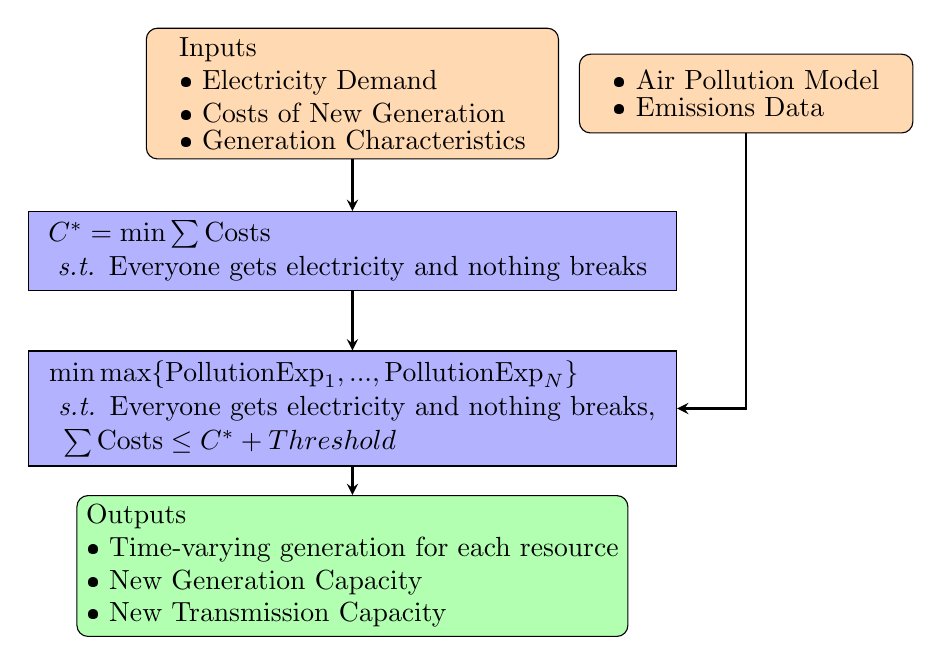
\begin{tikzpicture}[node distance=2cm]

\node (start) [start, text width=5cm] {\shortstack[l]{Inputs\\• Electricity Demand \\ • Costs of New Generation \\ • Generation Characteristics}};

\node (air) [start, text width=4cm, right of= start, xshift=3cm] {\shortstack[l]{• Air Pollution Model\\
• Emissions Data}};

\node(obj)[process, below of=start, text width=8cm, xshift=0cm]{\shortstack[l]{$C^* = \min \sum \text{Costs}$ \\ \textit{ 
   s.t.   }\text{Everyone gets electricity and nothing breaks }}};

\node(obj2)[process, below of=obj, text width=8cm, xshift=0cm]{\shortstack[l]{$\min \max\{\text{PollutionExp}_1,...,\text{PollutionExp}_N\}$ \\ \textit{ 
   s.t.   }\text{Everyone gets electricity and nothing breaks,} \\
    $\text{      }\sum \text{Costs} \leq C^*+Threshold$ }};

\node (result) [stop, below of=obj2] {\shortstack[l]{Outputs\\• Time-varying generation for each resource \\ • New Generation Capacity \\ • New Transmission Capacity}};

\draw [arrow] (start) -- (obj);
\draw [arrow] (air) |- (obj2);
\draw [arrow] (obj) -- (obj2);
\draw [arrow] (obj2) -- (result);


\end{tikzpicture}
\caption{Our Modification to the Least-Cost Planning Model}
\end{center}
\end{figure}

\section{Results}
\subsection{Model Inputs}
There are a few findings from the construction of model inputs that are worth discussing. First, unsurprisingly, empirical data on emissions and generation reveals that coal is a dirty source of generation. However, when we translate emissions into marginal exposure coefficients, we find that the average relative difference between coal and natural gas decreases. In particular, it appears that natural gas plants are on average, closer to Asian and Latino population centers. A unit of electricity generated from coal only causes slightly more damage (in terms of population-weighted PM2.5 exposure) to Asians and Latinos than a unit of electricity generated from natural gas. In figure \ref{EmissionsExposureCoefs} we plot the average empirical emissions rates by technology in panel (a), and the mean coefficients describing how one MWh of generation affects mean group-level exposure of PM2.5 in $\mu$g/m$^3$. 

This stark divergence between the relative emissions rates and the relative exposure coefficients highlights one of the central premises of the paper -- that where generation is placed can have large impacts on pollution exposure, and that selectively choosing what generation goes where can lead to large decreases in pollution exposure at low costs.

\begin{figure}
\centering
\subcaptionbox{Mean empirical emissions rates by technology in tons per MWh.}{\includegraphics[width=0.8\textwidth]{Figures/EndogenousPaper/emissions_by_technology.png}}%
\hfill
\subcaptionbox{Mean coefficients describing how a marginal MWh of generation affects mean group-level PM2.5 exposure.}{\includegraphics[width=0.8\textwidth]{Figures/EndogenousPaper/exposure_by_technology.png}}%
\hfill
\caption{Coal is far dirtier than other technologies when looking at emissions rates (Tons/MWh).  However, the discrepancy between technologies is more narrow for exposure, reflecting differences across the technologies in their spatial distribution.}
\label{EmissionsExposureCoefs}
\end{figure}

\subsection{Model Results}
Our high-level, key finding is that even a modest budget of $\$50$ billion through 2050 could pay for massive reductions in equitable air quality improvement. For context, the total system costs in the base scenario are about $\$2.4$ trillion, so $\$50$ billion represents an increase in total costs of about 2$\%$. In the $\$50$ billion budget scenario, the maximum group level exposures are approximately cut in half in each model period relative to the base scenario. 

Our results have features that you would expect based on economic theory. In figure \ref{PPF}, we plot the maximum group exposure in each model period against the budget for reducing pollution. There are increasing costs of reducing air pollution -- in other words, the gains from moving from least-cost to allocating $\$50$ billion to reduce pollution exposure are much larger than the gains from moving from allocating $\$50$ billion to $\$100$ billion.

\begin{figure}
    \centering
    \includegraphics[width=0.7\linewidth]{Figures/EndogenousPaper/exposure_cost_PPF.png}
    \caption{The relationship between the objective function (min-max of exposure in $\mug$/MWh) and the cost limit constraint.}
    \label{PPF}
\end{figure}

In figure \ref{ExposureByRace} we've plotted mean exposure by race across different budgets in the year 2050 model period. Our results show that the groups with the highest baseline exposures -- Black, Asian, and Latino Americans experience the greatest gains from the scenarios which reduce air pollution. Our results also suggest that at the optimum, the min-max objective generates equal average exposures for most groups. In other words, the min-max function binds for most groups.

\begin{figure}
    \centering
    \includegraphics[width=0.5\linewidth]{Figures/EndogenousPaper/exposure_by_scenario_2050.png}
    \caption{Population-weighted mean air pollution exposure by race in 2050 across budget scenarios.}
    \label{ExposureByRace}
\end{figure}

\subsection{Mechanisms}

The model primarily produces air pollution benefits by shifting away from fossil generation towards zero-emissions, renewable generation. In figure \ref{Generation}, we've plotted annual generation from different technologies, by budget scenario and model year.

\begin{figure}
    \centering
    {\includegraphics[width=0.45\textwidth]{Figures/EndogenousPaper/Dispatch_Relative_by_scenario_2027.png}}
    {\includegraphics[width=0.45\textwidth]{Figures/EndogenousPaper/Dispatch_Relative_by_scenario_2030.png}}\\
    {\includegraphics[width=0.45\textwidth]{Figures/EndogenousPaper/Dispatch_Relative_by_scenario_2035.png}}
    {\includegraphics[width=0.45\textwidth]{Figures/EndogenousPaper/Dispatch_Relative_by_scenario_2040.png}}\\
    {\includegraphics[width=0.45\textwidth]{Figures/EndogenousPaper/Dispatch_Relative_by_scenario_2045.png}}
    {\includegraphics[width=0.45\textwidth]{Figures/EndogenousPaper/Dispatch_Relative_by_scenario_2050.png}}\\
    \includegraphics[width=0.45\textwidth]{Figures/EndogenousPaper/Legend_2050.png}
    \caption{Generation from each technology category across scenario-years.}
    \label{Generation}

\end{figure}

In the nearer-term, the model chooses to replace almost all existing coal generation with natural gas and wind generation. Note that in 2050, even in the base scenario, the cost-minimizing model almost entirely pushes out coal. So, one major thing the model spends its budget on when trying to reduce pollution exposure is getting rid of coal sooner, especially in the mid-Atlantic and Midwest regions. We've plotted the difference between generation from coal in the base and $\$200$ billion scenario in figure \ref{coalmap}.
\begin{figure}
    \centering
    \includegraphics[width=0.8\linewidth]{Figures/EndogenousPaper/coal_generation_map_2027_200B.png}
    \caption{Difference in coal generation in 2027 with $\$200$ billion budget relative to the base scenario}
    \label{coalmap}
\end{figure}

In the far-term, the model broadly chooses to replace natural gas with wind and solar. In figure \ref{2050Generation} we plot differences in natural gas, wind, and solar generation. However, rather than decreasing natural gas use across the board, the model instead chooses to sharply reduce natural gas generation in some regions, such as eastern Texas, southern California, the Midwest, and the northern Mid-Atlantic, while modestly increasing natural gas generation in other areas like west Texas and the Pacific Northwest.

\begin{figure}
    \centering
    \includegraphics[width=0.8\linewidth]{Figures/EndogenousPaper/naturalgas_generation_map.png}
    \includegraphics[width=0.8\linewidth]{Figures/EndogenousPaper/wind_generation_map.png}
    \includegraphics[width=0.8\linewidth]{Figures/EndogenousPaper/solar_generation_map.png}
    \caption{Differences in generation from natural gas, wind, and solar in 2050 with a $\$200$ billion budget relative to the base scenario}
    \label{2050Generation}
\end{figure}

In a few areas, the model uses transmission as a way to decrease air pollution. In figure \ref{transmissionsubstitution}, we've plotted an example of how this works. To reduce air pollution, the model over-constructs capacity in some regions, in this example, southern part of the Southwest Power Pool (SPP), and allows that region to export to adjacent areas.

\begin{figure}
    \centering
    \includegraphics[width=0.9\linewidth]{Figures/EndogenousPaper/transmission_capacity_substitution.png}
    \caption{Differences in Transmission and Generation Capacity Relative to the Base Scenario}
    \label{transmissionsubstitution}
\end{figure}

\subsection{Discussion}
While we think these results have important policy implications, namely that pollution exposure can be dramatically reduced at low costs, it's important to note that our results don't point to which policies would achieve the optimal solution. Rather, these results are prescriptive -- \textit{"Build X, Y, and Z in regions A,B, and C to achieve the deepest equitable cuts in air pollution at a certain cost."} However, these results could point towards policies which might approximate model results, such as targeted plant retirements or regional clean energy standards.

While our results are new, we think it's important to contextualize them with other findings from the literature. For example, \citet{Shawhan2024PoliciesAmericans} and \citet{Goforth2022AirStrategies} find that the U.S. is on track to dramatically reduce pollution exposure, and that faster decarbonization policies will generate deep cuts in air pollution exposure. Our results are broadly consistent with these findings. For example, in the base, current policies scenario, we predict that Black Americans will experience the largest drop in pollution exposures over the study period-- a decrease of about 50$\%$ between 2027 and 2050.

These results are somewhat unsurprising given the tight link between carbon emissions and pollution emissions. In figure \


\begin{figure}
    \centering
    \includegraphics[width=0.5\linewidth]{Figures/EndogenousPaper/emissions_vs_exposure.png}
    \caption{Caption}
    \label{emissionsexposure}
\end{figure}
\section{Conclusion}
This paper develops and applies a novel framework for integrating air pollution equity into electricity planning models. Rather than optimizing purely for cost or incorporating pollution as a monetized externality, we directly embed pollution exposure—measured in terms of group-specific PM2.5 burden—into the objective function using a Rawlsian min-max approach. We combine empirical emissions data, an atmospheric dispersion model (InMAP), and a least-cost power system optimization model (Switch) to identify power sector investments that minimize the maximum pollution burden across racial groups, all while remaining within a specified system cost constraint.

Our results demonstrate that substantial improvements in both aggregate and distributional air quality outcomes are achievable with relatively modest expenditures. For example, a $\$50$ billion investment—spread across several decades—can cut maximum group-level exposures in half relative to the least-cost baseline. The gains are not evenly distributed: Black, Latino, and Asian populations, who face the highest baseline exposures, benefit most from the model’s pollution-reduction strategies. Mechanistically, these improvements are achieved by accelerating coal retirements, strategically reducing natural gas generation in densely populated or upwind areas, increasing renewable deployment, and upgrading transmission infrastructure to allow for cleaner electricity imports.

Importantly, our modeling framework is prescriptive, not predictive. It does not identify specific policies, incentives, or mandates that would deliver the modeled outcomes. Instead, it provides a decision-support tool to help planners and policymakers understand the cost–equity tradeoffs embedded in electricity system design. As such, it complements—but does not replace regulatory or political processes.

This framework is generalizable. While we focus on air pollution equity, the same structure could be used to minimize job losses in vulnerable communities, optimize energy affordability across income groups, or equitably distribute benefits like clean energy jobs or infrastructure investment. Future work could extend this framework to include multiple dimensions of equity simultaneously or explore how it interacts with climate targets and carbon pricing. In sum, our work shows that by modifying standard electricity planning tools to account for pollution exposure and equity, it is possible to design cleaner, more equitable power systems at a reasonable cost.







\begin{singlespace}
\newpage
\bibliographystyle{jpe}
%\bibliographystyle{econometrica}
\bibliography{references.bib}
\end{singlespace}

\section{Appendix}
\end{document}  